% Ask the Sensors -- 10-minute presentation.
% Build: cd docs/slides && pdflatex slides.tex && pdflatex slides.tex
% Every number here comes from the same committed result files as the report.
\documentclass[aspectratio=169,11pt]{beamer}
\usepackage[T1]{fontenc}
\usepackage{lmodern}
\usepackage{microtype}
\usepackage{array}
\usepackage{booktabs}
\usepackage{tikz}
\usetikzlibrary{positioning,arrows.meta,decorations.pathreplacing,shapes.geometric}
\usepackage{graphicx}
\graphicspath{{../../results/}}

\definecolor{atsblue}{HTML}{2A78D6}
\definecolor{atsorange}{HTML}{EB6834}
\definecolor{atsgrey}{HTML}{4A4A4A}

\usetheme{default}
\usecolortheme{default}
\setbeamertemplate{navigation symbols}{}
\setbeamercolor{structure}{fg=atsblue}
\setbeamercolor{frametitle}{fg=white,bg=atsblue}
\setbeamerfont{frametitle}{size=\large,series=\bfseries}
\setbeamertemplate{frametitle}{%
  \nointerlineskip
  \begin{beamercolorbox}[wd=\paperwidth,ht=2.6ex,dp=1.2ex,leftskip=0.3cm,rightskip=0.3cm]{frametitle}
    \usebeamerfont{frametitle}\insertframetitle
  \end{beamercolorbox}
}
\setbeamertemplate{itemize item}{\color{atsblue}$\bullet$}
\setbeamertemplate{itemize subitem}{\color{atsorange}--}
\setbeamertemplate{footline}{%
  \hfill\usebeamerfont{footline}\color{atsgrey}\scriptsize
  Ask the Sensors\quad\insertframenumber/\inserttotalframenumber\hspace*{0.3cm}\vspace*{0.15cm}
}
\setbeamercolor{block title}{bg=atsblue!12,fg=atsblue}
\setbeamercolor{block body}{bg=atsblue!5}
\newcommand{\code}[1]{\texttt{\small #1}}
\newcommand{\hilite}[1]{\textcolor{atsorange}{\textbf{#1}}}

\title{\textbf{Ask the Sensors}}
\subtitle{Answering questions about daily activity from motion sensors, with evidence}
\author{Abhinav Kumar Singh (22CS30005) \and Harsh Chattar (22CS30028)}
\institute{CS60055 Ubiquitous Computing --- IIT Kharagpur\\Hackathon Challenge 1}
\date{}

\begin{document}

% ---------------------------------------------------------------- 1
\begin{frame}[plain]
  \vfill
  \begin{center}
    {\fontsize{38}{42}\selectfont\bfseries ASK THE SENSORS}

    \vspace{0.6em}
    {\large\color{atsgrey} Answering questions on sensor data, with evidence}

    \vspace{1.6em}
    {\normalsize\bfseries CS60055 Ubiquitous Computing}

    \vspace{0.25em}
    {\small\bfseries Hackathon Challenge 1}

    \vspace{1.4em}
    {\normalsize\color{atsgrey} Presented by}

    \vspace{0.7em}
    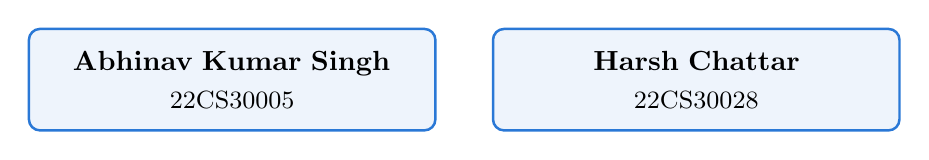
\begin{tikzpicture}[
      card/.style={draw=atsblue, line width=0.9pt, fill=atsblue!8, rounded corners=4pt,
                   align=center, text width=4.6cm, inner sep=8pt}]
      \node[card] (a) {\bfseries Abhinav Kumar Singh\\[0.15em] \small\mdseries 22CS30005};
      \node[card, right=0.7cm of a] (b) {\bfseries Harsh Chattar\\[0.15em] \small\mdseries 22CS30028};
    \end{tikzpicture}
  \end{center}
  \vfill
\end{frame}

% ---------------------------------------------------------------- 2
\begin{frame}[fragile]{The problem}
  \textbf{Scenario.}
  An older woman lives alone. She has a phone that carries motion sensors. Her
  son and her physiotherapist want to know how she is doing, based on the data
  those sensors record. We need to build a tool that answers their questions in
  \hilite{plain English} and also \hilite{provides the evidence} behind each
  answer.

  \medskip
  \textbf{What the tool must produce} --- the example given in the challenge
  brief:

  \smallskip
  \begin{center}
  \begin{minipage}{0.86\textwidth}
  \footnotesize
\begin{verbatim}
Query: "How long was the user walking?"
Answer: 700 seconds
Activity/Event: Walking
Evidence:
    Timestamp(s): 905 to 1420, 2110 to 2295 (seconds from start)
    Sensor Modality: Accelerometer, Gyroscope
    Sensor Channel(s): All
Explanation: Walking was detected in two separate intervals, of 515 and 185
             seconds, which sum to 700 seconds.
\end{verbatim}
  \end{minipage}
  \end{center}

  \smallskip
  \small
  Not just \emph{``700 seconds''} --- but \hilite{which stretches of signal},
  from \hilite{which sensors}, and \hilite{why} they read as walking.
\end{frame}

% ---------------------------------------------------------------- 3
\begin{frame}{Functional requirements: four question tiers, one system}
  \footnotesize
  The evaluation mixes all four tiers, without saying which is which.
  \smallskip

  {\scriptsize\renewcommand{\arraystretch}{1.2}
  \begin{tabular}{@{}>{\raggedright\arraybackslash}p{0.19\textwidth}
                    >{\raggedright\arraybackslash}p{0.40\textwidth}
                    >{\raggedright\arraybackslash}p{0.35\textwidth}@{}}
    \toprule
    \textbf{Tier} & \textbf{Example question} & \textbf{What must be produced} \\
    \midrule
    \textbf{1. Identification} &
    ``What activity is she performing?''\newline ``Is she running?'' &
    The activity, or a yes/no verdict \\[0.35em]
    \textbf{2. Temporal \& quantitative} &
    ``How long was she walking?''\newline ``How many times?'' &
    Numbers computed across the \emph{whole} recording, with intervals \\[0.35em]
    \textbf{3. Evidence grounding} &
    ``Did she begin running, and when?'' &
    Answer \emph{plus} timestamps, sensor modality, channels, and the reasoning \\[0.35em]
    \textbf{4. Open-world reasoning} &
    ``Was she resting for a long time?''\newline ``Was she fidgeting?'' &
    A verdict on behaviour \emph{outside} the seven trained labels, argued from the signal \\
    \bottomrule
  \end{tabular}}

  \smallskip
  \begin{columns}[T,onlytextwidth]
    \begin{column}{0.48\textwidth}
      \begin{block}{The seven activities we recognise}
        Lying, sitting, standing in place, standing and moving, walking,
        running, bicycling.
      \end{block}
    \end{column}
    \begin{column}{0.48\textwidth}
      \begin{block}{One fixed output format, every tier}
        Answer, activity/event, evidence (timestamps, modality, channels),
        explanation. \code{N/A} is the only permitted blank.
      \end{block}
    \end{column}
  \end{columns}
\end{frame}

% ---------------------------------------------------------------- 4
\begin{frame}{Architecture: two halves, one agreed file}
  \vfill
  \begin{center}
  \resizebox{\textwidth}{!}{%
  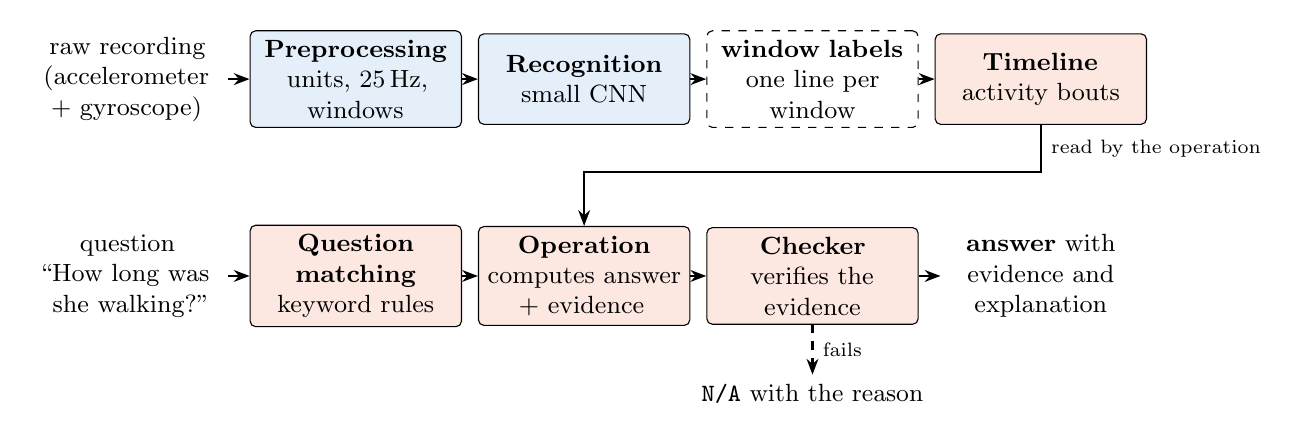
\begin{tikzpicture}[
    sig/.style={draw, rounded corners=2pt, fill=atsblue!12, align=center, font=\small, minimum height=1.15cm, text width=2.45cm},
    ans/.style={draw, rounded corners=2pt, fill=atsorange!15, align=center, font=\small, minimum height=1.15cm, text width=2.45cm},
    io/.style={align=center, font=\small, text width=2.3cm},
    arr/.style={-{Stealth[length=2mm]}, thick}]
  \node[io]  (rec)  at (0,0)      {raw recording\\(accelerometer + gyroscope)};
  \node[sig] (pre)  at (2.9,0)    {\textbf{Preprocessing}\\units, 25\,Hz, windows};
  \node[sig] (cnn)  at (5.8,0)    {\textbf{Recognition}\\small CNN};
  \node[draw, dashed, rounded corners=2pt, align=center, font=\small, minimum height=1.15cm, text width=2.45cm] (file) at (8.7,0) {\textbf{window labels}\\one line per window};
  \node[ans] (tl)   at (11.6,0)   {\textbf{Timeline}\\activity bouts};
  \node[io]  (q)    at (0,-2.5)   {question\\``How long was she walking?''};
  \node[ans] (rt)   at (2.9,-2.5) {\textbf{Question matching}\\keyword rules};
  \node[ans] (op)   at (5.8,-2.5) {\textbf{Operation}\\computes answer + evidence};
  \node[ans] (chk)  at (8.7,-2.5) {\textbf{Checker}\\verifies the evidence};
  \node[io]  (out)  at (11.6,-2.5){\textbf{answer} with evidence and explanation};
  \node[font=\small] (na) at (8.7,-4.0) {\code{N/A} with the reason};
  \draw[arr] (rec) -- (pre); \draw[arr] (pre) -- (cnn); \draw[arr] (cnn) -- (file); \draw[arr] (file) -- (tl);
  \draw[arr] (q) -- (rt); \draw[arr] (rt) -- (op); \draw[arr] (op) -- (chk); \draw[arr] (chk) -- (out);
  \draw[arr] (tl.south) -- node[right, font=\scriptsize]{read by the operation} ++(0,-0.6) -| (op.north);
  \draw[arr, dashed] (chk) -- node[right, font=\scriptsize]{fails} (na);
  \end{tikzpicture}}
  \end{center}
  \vfill
\end{frame}

% ---------------------------------------------------------------- 5
\begin{frame}{Recognition: a deliberately small network}
  \begin{center}
  \resizebox{\textwidth}{!}{%
  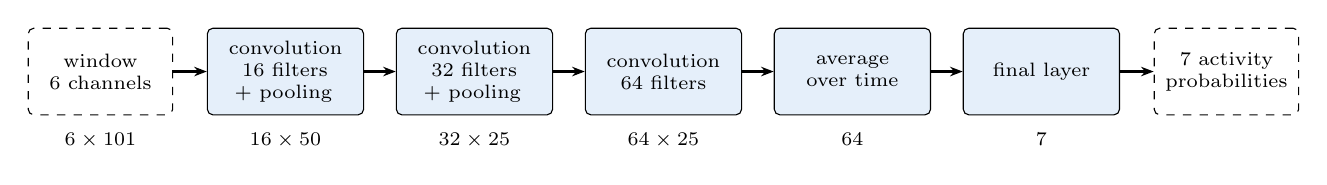
\begin{tikzpicture}[
    layer/.style={draw, rounded corners=2pt, fill=atsblue!12, align=center, font=\scriptsize, minimum height=1.1cm, text width=1.75cm},
    dims/.style={font=\scriptsize\itshape, align=center},
    arr/.style={-{Stealth[length=1.6mm]}, thick}]
  \node[draw, dashed, rounded corners=2pt, align=center, font=\scriptsize, minimum height=1.1cm, text width=1.6cm] (in) at (0,0) {window\\6 channels};
  \node[layer] (c1) at (2.35,0)  {convolution\\16 filters\\+ pooling};
  \node[layer] (c2) at (4.75,0)  {convolution\\32 filters\\+ pooling};
  \node[layer] (c3) at (7.15,0)  {convolution\\64 filters};
  \node[layer] (gp) at (9.55,0)  {average\\over time};
  \node[layer] (fc) at (11.95,0) {final layer};
  \node[draw, dashed, rounded corners=2pt, align=center, font=\scriptsize, minimum height=1.1cm, text width=1.6cm] (out) at (14.3,0) {7 activity\\probabilities};
  \foreach \a/\b in {in/c1, c1/c2, c2/c3, c3/gp, gp/fc, fc/out} { \draw[arr] (\a) -- (\b); }
  \node[dims, below=0.1cm of in] {$6 \times 101$};
  \node[dims, below=0.1cm of c1] {$16 \times 50$};
  \node[dims, below=0.1cm of c2] {$32 \times 25$};
  \node[dims, below=0.1cm of c3] {$64 \times 25$};
  \node[dims, below=0.1cm of gp] {$64$};
  \node[dims, below=0.1cm of fc] {$7$};
  \end{tikzpicture}}
  \end{center}
  \vspace{-0.2em}
  \begin{columns}[T,onlytextwidth]
    \begin{column}{0.53\textwidth}
      \small
      \textbf{Input.} A 4-second window, a new one every 2 seconds:
      $6$ channels $\times$ $101$ samples at 25\,Hz.

      \smallskip
      \textbf{Why so small?} \hilite{9{,}975 parameters, 48\,KB} --- it runs on a
      phone and compresses cleanly (slide 9).

      \smallskip
      \textbf{Trained} on 36 people, validated on 12 others; nobody appears in
      both. Rare activities are weighted up (running is 0.6\% of windows).

      \smallskip
      \textbf{Result.} macro-F1 \hilite{0.289}, against 0.079 (always guess the
      commonest activity) and 0.225 (logistic regression).
    \end{column}
    \begin{column}{0.45\textwidth}
      \includegraphics[width=\linewidth]{fig2_confusion_matrix.png}
    \end{column}
  \end{columns}
\end{frame}

% ---------------------------------------------------------------- 6
\begin{frame}{Answering and checking: where grounding is enforced}
  \footnotesize
  \begin{block}{The rule that shapes the whole design}
    A language model \hilite{never} produces a number, an interval or a verdict.
    Every quantity is computed in ordinary code from the timeline, so it can be
    recomputed and checked. The small language model we tested chooses only
    \emph{which operation runs}; it never sees the signal.
  \end{block}
  \begin{columns}[T,onlytextwidth]
    \begin{column}{0.55\textwidth}
      \textbf{1. Match} the question to one of eight operations:
      \smallskip

      \begin{tabular}{@{}ll@{}}
        \toprule
        Operation & Example \\
        \midrule
        Identify      & ``What was she doing at 340\,s?'' \\
        Verify        & ``Is she running?'' \\
        Duration      & ``How long was she walking?'' \\
        Count         & ``How many times did she walk?'' \\
        Compare       & ``More time walking or running?'' \\
        Find start    & ``When did she begin running?'' \\
        Show evidence & ``Cite the evidence for walking.'' \\
        Open-ended    & ``Was she resting for a long time?'' \\
        \bottomrule
      \end{tabular}

      \smallskip
      \textbf{2. Compute} the answer and the intervals behind it, quoting the
      measured signal in the explanation.
    \end{column}
    \begin{column}{0.43\textwidth}
      \textbf{3. Check} --- before anything is shown:
      \begin{itemize}
        \item every cited interval \hilite{exists} in the timeline;
        \item the printed times \hilite{match} those intervals;
        \item tiers that need evidence \hilite{have} it;
        \item durations and counts \hilite{add up again} from the intervals.
      \end{itemize}

      \smallskip
      A failing answer is withheld and replaced by \code{N/A} with the reason.
      There is no bypass.

      \smallskip
      \textbf{Open-world questions} rest on measured stillness, not on labels.
    \end{column}
  \end{columns}
\end{frame}

% ---------------------------------------------------------------- 7
\begin{frame}[fragile]{Real output: four questions, one recording}
  \scriptsize
  \begin{columns}[T,onlytextwidth]
    \begin{column}{0.49\textwidth}
      \textcolor{atsblue}{\textbf{Tier 1 --- identification}}
\begin{verbatim}
Query: "What activity ... at 340 seconds?"
Answer:          Sitting
Activity/Event:  Sitting
Evidence:
  Timestamp(s):  0 to 600 (seconds from start)
  Modality:      Accelerometer, Gyroscope
  Channel(s):    All
Explanation:     340 s falls inside 0-600 s,
  classified as sitting (confidence 0.85);
  100 windows, mean 9.80 m/s^2, std 0.08.
\end{verbatim}
      \medskip
      \textcolor{atsblue}{\textbf{Tier 2 --- duration}}
\begin{verbatim}
Query: "How long was the user walking?"
Answer:          720 seconds
Evidence:
  Timestamp(s):  600 to 1080, 1320 to 1560
Explanation:     Walking was detected in 2
  interval(s) of 480, 240 s, summing to
  720 s; cadence near 1.90 Hz in 100% of
  windows.
\end{verbatim}
    \end{column}
    \begin{column}{0.49\textwidth}
      \textcolor{atsblue}{\textbf{Tier 3 --- evidence grounding}}
\begin{verbatim}
Query: "Did the user begin walking, when?"
Answer:          Yes, walking began at 600 s
Activity/Event:  Onset of walking
Evidence:
  Timestamp(s):  600 to 1080
Explanation:     The first walking interval
  runs 600-1080 s, following sitting; across
  the transition accelerometer std goes
  0.08 -> 1.55 m/s^2 and gyroscope energy
  0.124 -> 1.45.
\end{verbatim}
      \medskip
      \textcolor{atsorange}{\textbf{Tier 4 --- refusing to guess}}
\begin{verbatim}
Query: "Was the user driving?"
Answer:          N/A
Evidence:        N/A
Explanation:     This question does not match
  any reasoning pattern the system supports,
  and answering it would mean guessing beyond
  the recorded evidence.
\end{verbatim}
    \end{column}
  \end{columns}
  \centering\tiny
  Verbatim system output; explanations trimmed to fit.
\end{frame}

% ---------------------------------------------------------------- 8
\begin{frame}{What we did differently (1): grounding, and a timeline that fits the data}
  \begin{columns}[T,onlytextwidth]
    \begin{column}{0.48\textwidth}
      \centering
      \resizebox{\linewidth}{!}{%
      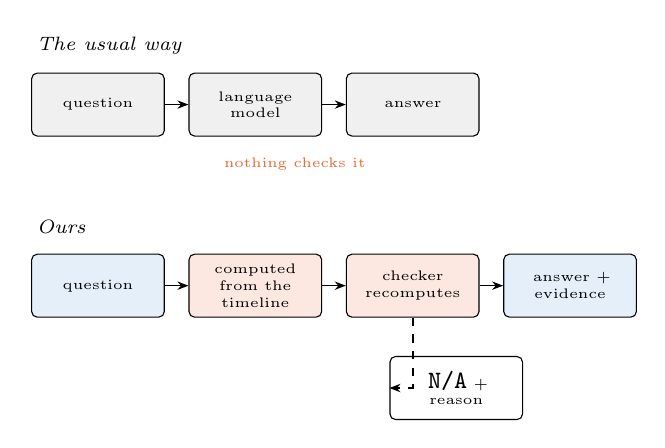
\begin{tikzpicture}[
        b/.style={draw, rounded corners=2pt, align=center, font=\tiny, minimum height=0.8cm, text width=1.45cm},
        arr/.style={-{Stealth[length=1.4mm]}, semithick}]
      \node[font=\scriptsize\itshape, anchor=west] at (-0.1,1.75) {The usual way};
      \node[b, fill=gray!12] (q1) at (0.8,1.0) {question};
      \node[b, fill=gray!12, right=0.3cm of q1] (m1) {language model};
      \node[b, fill=gray!12, right=0.3cm of m1] (a1) {answer};
      \draw[arr] (q1) -- (m1); \draw[arr] (m1) -- (a1);
      \node[font=\tiny, text=atsorange] at (3.3,0.25) {nothing checks it};
      \node[font=\scriptsize\itshape, anchor=west] at (-0.1,-0.55) {Ours};
      \node[b, fill=atsblue!12] (q2) at (0.8,-1.3) {question};
      \node[b, fill=atsorange!15, right=0.3cm of q2] (op2) {computed from the timeline};
      \node[b, fill=atsorange!15, right=0.3cm of op2] (ck2) {checker recomputes};
      \node[b, fill=atsblue!12, right=0.3cm of ck2] (a2) {answer + evidence};
      \draw[arr] (q2) -- (op2); \draw[arr] (op2) -- (ck2); \draw[arr] (ck2) -- (a2);
      \node[b, fill=white, font=\tiny] (na2) at (5.35,-2.6) {\code{N/A} + reason};
      \draw[arr, dashed] (ck2) |- (na2);
      \end{tikzpicture}}

      \smallskip
      \footnotesize
      \textbf{Grounding by construction.} Every number and interval is
      recomputed before release; anything that fails is withheld.
      \hilite{An ungrounded answer is structurally impossible}, not just
      unlikely.
    \end{column}
    \begin{column}{0.48\textwidth}
      \centering
      \resizebox{\linewidth}{!}{%
      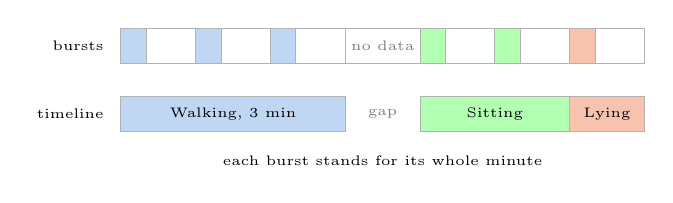
\begin{tikzpicture}[x=0.95cm, y=0.75cm]
      \foreach \i in {0,...,6} { \draw[gray!60] (\i,1.15) rectangle ++(1,0.6); }
      \foreach \i/\col in {0/atsblue!30, 1/atsblue!30, 2/atsblue!30, 4/green!30, 5/green!30, 6/atsorange!40} {
        \draw[fill=\col, draw=gray!60] (\i,1.15) rectangle ++(0.34,0.6);
      }
      \node[font=\tiny, text=gray] at (3.5,1.45) {no data};
      \draw[fill=atsblue!30, draw=gray!60] (0,0) rectangle (3,0.6);
      \node[font=\tiny] at (1.5,0.3) {Walking, 3 min};
      \node[font=\tiny, text=gray] at (3.5,0.3) {gap};
      \draw[fill=green!30, draw=gray!60] (4,0) rectangle (6,0.6);
      \node[font=\tiny] at (5,0.3) {Sitting};
      \draw[fill=atsorange!40, draw=gray!60] (6,0) rectangle (7,0.6);
      \node[font=\tiny] at (6.5,0.3) {Lying};
      \node[font=\tiny, anchor=east] at (-0.1,1.45) {bursts};
      \node[font=\tiny, anchor=east] at (-0.1,0.3) {timeline};
      \node[font=\tiny, anchor=north] at (3.5,-0.25) {each burst stands for its whole minute};
      \end{tikzpicture}}

      \smallskip
      \footnotesize
      \textbf{A timeline that fits the data.} The phone records about 20\,s per
      labelled minute. Summing windows would report \hilite{a third of reality};
      bridging clock drift turned \hilite{3{,}151 fragments into 325 real bouts}.
    \end{column}
  \end{columns}
\end{frame}

% ---------------------------------------------------------------- 9
\begin{frame}{What we did differently (2): tracing errors, and untrained behaviours}
  \begin{columns}[T,onlytextwidth]
    \begin{column}{0.48\textwidth}
      \centering
      \resizebox{\linewidth}{!}{%
      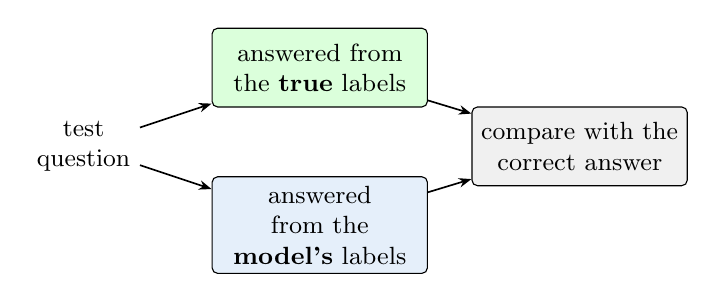
\begin{tikzpicture}[
        b/.style={draw, rounded corners=2pt, align=center, font=\small, minimum height=1.0cm, text width=2.5cm},
        arr/.style={-{Stealth[length=1.6mm]}, semithick}]
      \node[align=center, font=\small] (q) at (0,0) {test\\question};
      \node[b, fill=green!14] (t) at (3.0,1.0) {answered from the \textbf{true} labels};
      \node[b, fill=atsblue!12] (m) at (3.0,-1.0) {answered from the \textbf{model's} labels};
      \node[b, fill=gray!12] (c) at (6.3,0) {compare with the correct answer};
      \draw[arr] (q) -- (t); \draw[arr] (q) -- (m);
      \draw[arr] (t) -- (c); \draw[arr] (m) -- (c);
      \end{tikzpicture}}

      \smallskip
      \footnotesize
      \textbf{Two tracks, identical code.} Right with true labels but wrong
      with the model's $\Rightarrow$ a \textbf{recognition} error; wrong either
      way $\Rightarrow$ an \textbf{answering} error. This is \emph{how} we can
      say \hilite{all 19 misses are recognition errors}.
    \end{column}
    \begin{column}{0.48\textwidth}
      \centering
      \resizebox{\linewidth}{!}{%
      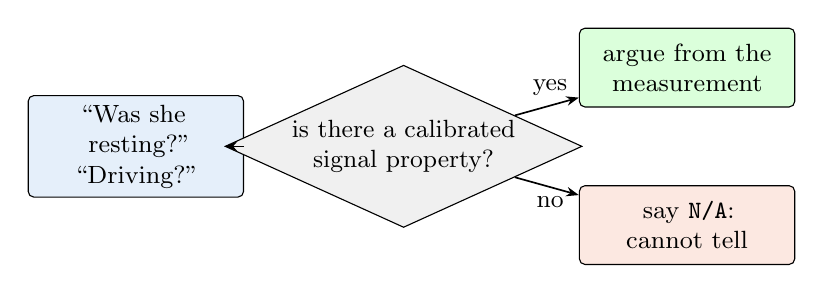
\begin{tikzpicture}[
        b/.style={draw, rounded corners=2pt, align=center, font=\small, minimum height=1.0cm, text width=2.5cm},
        d/.style={draw, diamond, aspect=2.2, align=center, font=\small, inner sep=1pt, fill=gray!12},
        arr/.style={-{Stealth[length=1.6mm]}, semithick}]
      \node[b, fill=atsblue!12] (q) at (0,0) {``Was she resting?''\\``Driving?''};
      \node[d] (dec) at (3.4,0) {is there a calibrated\\signal property?};
      \node[b, fill=green!14] (yes) at (7.0,1.0) {argue from the measurement};
      \node[b, fill=atsorange!15] (no) at (7.0,-1.0) {say \code{N/A}:\\cannot tell};
      \draw[arr] (q) -- (dec);
      \draw[arr] (dec) -- node[font=\small, above, pos=0.55] {yes} (yes);
      \draw[arr] (dec) -- node[font=\small, below, pos=0.55] {no} (no);
      \end{tikzpicture}}

      \smallskip
      \footnotesize
      \textbf{Untrained behaviours, still answered honestly.} Stillness is
      calibrated from data, with a per-recording gyroscope-bias correction ---
      and where no signature exists, the system \hilite{declines rather than
      guesses}.
    \end{column}
  \end{columns}

  \vspace{0.3em}
  \centering\footnotesize
  We also built the small-language-model path and \hilite{measured it losing}
  to keyword rules --- then reported that, rather than shipping the fancier option.
\end{frame}

% ---------------------------------------------------------------- 9
\begin{frame}{Results: the answering layer is not the bottleneck}
  \centering
  \includegraphics[height=0.68\textheight]{fig1_accuracy_by_question_type.png}

  \vspace{0.3em}
  \raggedright\scriptsize
  \begin{itemize}
    \item \textbf{True labels:} \hilite{87 of 87} questions correct.
    \item \textbf{Model's labels:} \hilite{15 of 34} (39\%) --- and
    \hilite{all 19 misses are recognition errors}, none from the answering
    layer.
    \item \textbf{Durations and counts collapse:} they accumulate per-minute
    errors over tens of hours.
    \item \textbf{Stress test:} mislabel 10\% of minutes and the score still
    holds at \hilite{84\%}.
  \end{itemize}
\end{frame}

% ---------------------------------------------------------------- 9
\begin{frame}{Efficiency: small to begin with, smaller after compression}
  \centering
  \includegraphics[height=0.62\textheight]{fig4_pareto.png}

  \vspace{0.3em}
  \raggedright\scriptsize
  \begin{itemize}
    \item \textbf{On the target laptop:} 9{,}975 parameters, 0.047\,MB,
    \hilite{0.40\,ms} per window, \hilite{67\,ms} per question.
    \item \textbf{Three compressed versions, no retraining:} 8-bit weights,
    30\%/60\% of filters removed.
    \item The 8-bit model is \hilite{27\% smaller at no accuracy cost};
    compression buys \emph{space}, not speed.
    \item \textbf{Robustness:} dropping half the raw samples costs almost
    nothing (0.393 $\rightarrow$ 0.375).
  \end{itemize}
\end{frame}


% ---------------------------------------------------------------- 12
\begin{frame}{Limitations, and how we used AI tools}
  \footnotesize
  \begin{columns}[T,onlytextwidth]
    \begin{column}{0.49\textwidth}
      \begin{block}{Limitations}
        \begin{itemize}
          \item \textbf{Recognition caps everything.} macro-F1 0.289 limits the
          system to 15 of 34 on real users, even though the answering layer
          made no errors.
          \item \textbf{Optimistic numbers.} Both real test users are in the
          training group; held-out users would do worse.
          \item \textbf{Small, self-written question sets} (87 questions), and
          a router tuned against phrasings we wrote ourselves.
          \item \textbf{Stillness is our only calibrated property;} other
          behaviours rely on labels or decline to answer.
          \item \textbf{Energy is an estimate}, not a meter reading, and only
          one kind of input damage was tested.
        \end{itemize}
      \end{block}
    \end{column}
    \begin{column}{0.49\textwidth}
      \begin{block}{Use of AI tools}
        \textbf{Inside the system.} Qwen2.5-0.5B as an optional question
        parser, and Claude Haiku 4.5 to score explanations during evaluation.
        Neither ever produces an answer the system gives.

        \smallskip
        \textbf{As development assistants.} Claude Code was used to help write
        and debug code and tests, to explain concepts and documentation, and to
        help draft the report.

        \smallskip
        We directed the work, made the design decisions, reviewed what the
        tools produced, and \hilite{checked every reported number by running
        our own code}.
      \end{block}
    \end{column}
  \end{columns}
\end{frame}

% ---------------------------------------------------------------- 13
\begin{frame}{Contributions}
  \centering
  \begin{columns}[T,onlytextwidth]
    \begin{column}{0.48\textwidth}
      \begin{block}{Abhinav Kumar Singh (22CS30005)}
        \footnotesize
        \textbf{The signal half.}
        \begin{itemize}
          \item Data download, parsing and per-phone unit detection
          \item Resampling to 25\,Hz, gap policy, windowing, subject splits
          \item The recognition model and its confusion analysis
          \item Cost measurement, model compression, robustness testing
        \end{itemize}
      \end{block}
    \end{column}
    \begin{column}{0.48\textwidth}
      \begin{block}{Harsh Chattar (22CS30028)}
        \footnotesize
        \textbf{The answering half.}
        \begin{itemize}
          \item The activity timeline and evidence attribution
          \item Question matching and the eight operations
          \item Signal-based answers for open-ended questions
          \item The checker that blocks unsupported answers
          \item The whole evaluation: test questions, scoring, error tracing
        \end{itemize}
      \end{block}
    \end{column}
  \end{columns}

  \vspace{0.5em}
  {\footnotesize Both halves meet at one frozen file format, which is why each
  could be built and tested independently.}
\end{frame}

% ---------------------------------------------------------------- 12
\begin{frame}[plain]
  \vfill
  \begin{center}
    {\fontsize{36}{40}\selectfont\bfseries THANK YOU}

    \vspace{1.0em}
    {\large\color{atsgrey} Questions?}

    \vspace{1.8em}
    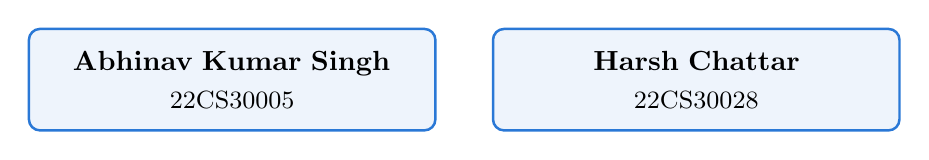
\begin{tikzpicture}[
      card/.style={draw=atsblue, line width=0.9pt, fill=atsblue!8, rounded corners=4pt,
                   align=center, text width=4.6cm, inner sep=8pt}]
      \node[card] (a) {\bfseries Abhinav Kumar Singh\\[0.15em] \small\mdseries 22CS30005};
      \node[card, right=0.7cm of a] (b) {\bfseries Harsh Chattar\\[0.15em] \small\mdseries 22CS30028};
    \end{tikzpicture}

    \vspace{1.2em}
    {\small\texttt{github.com/code-Harsh247/AskTheSensors}}
  \end{center}
  \vfill
\end{frame}

\end{document}
